\documentclass[12pt,a4paper]{nsiarticle}
\pagestyle{empty}
\begin{document}
\titre{Non Transitive Dice}
\classe{Euro 1\ere}
\maketitle
Look at the three dice below. They do not have values 1 to 6 like normal dice. 
In fact each die\footnote{die is singular, dice is plural
} is distinct.\\
We can play a two-player game in which each player picks a die and then rolls it. The player who has the
highest value on his die wins. For example, a 6 on the red die beats a 2 on the blue die. 
\begin{center}
    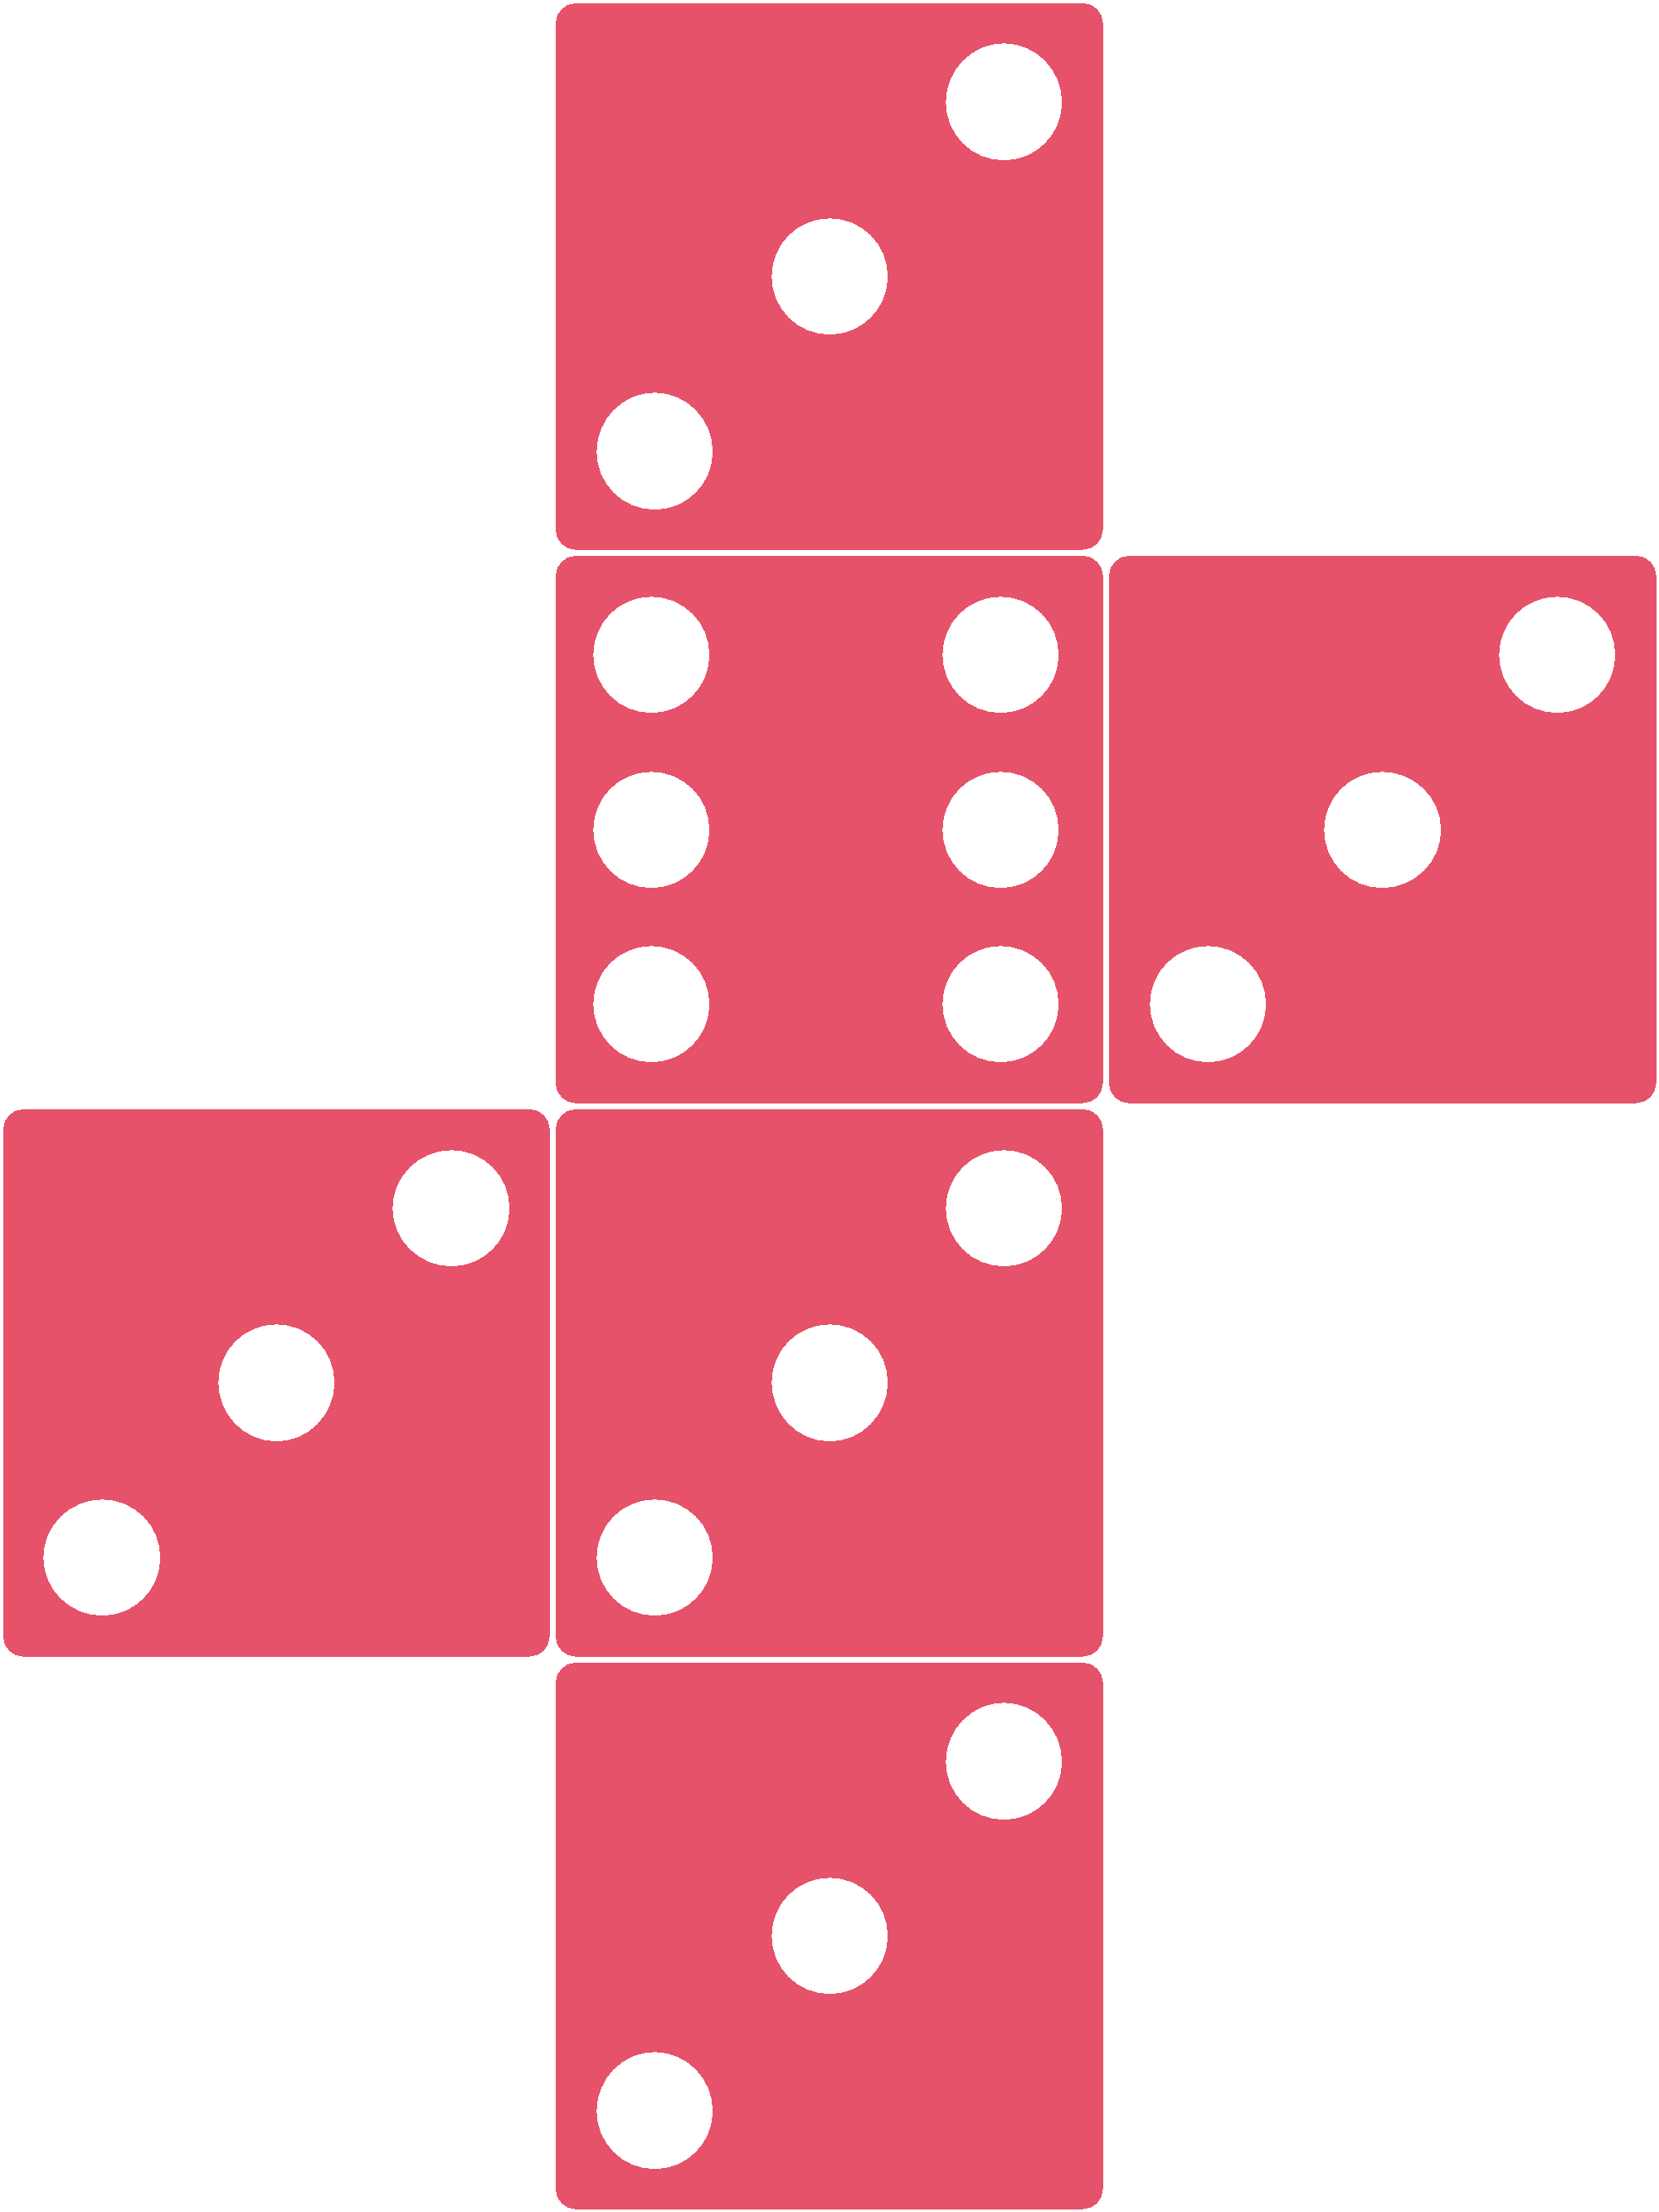
\includegraphics[width=4cm]{img/red_die.png}
    \hspace{1cm}
    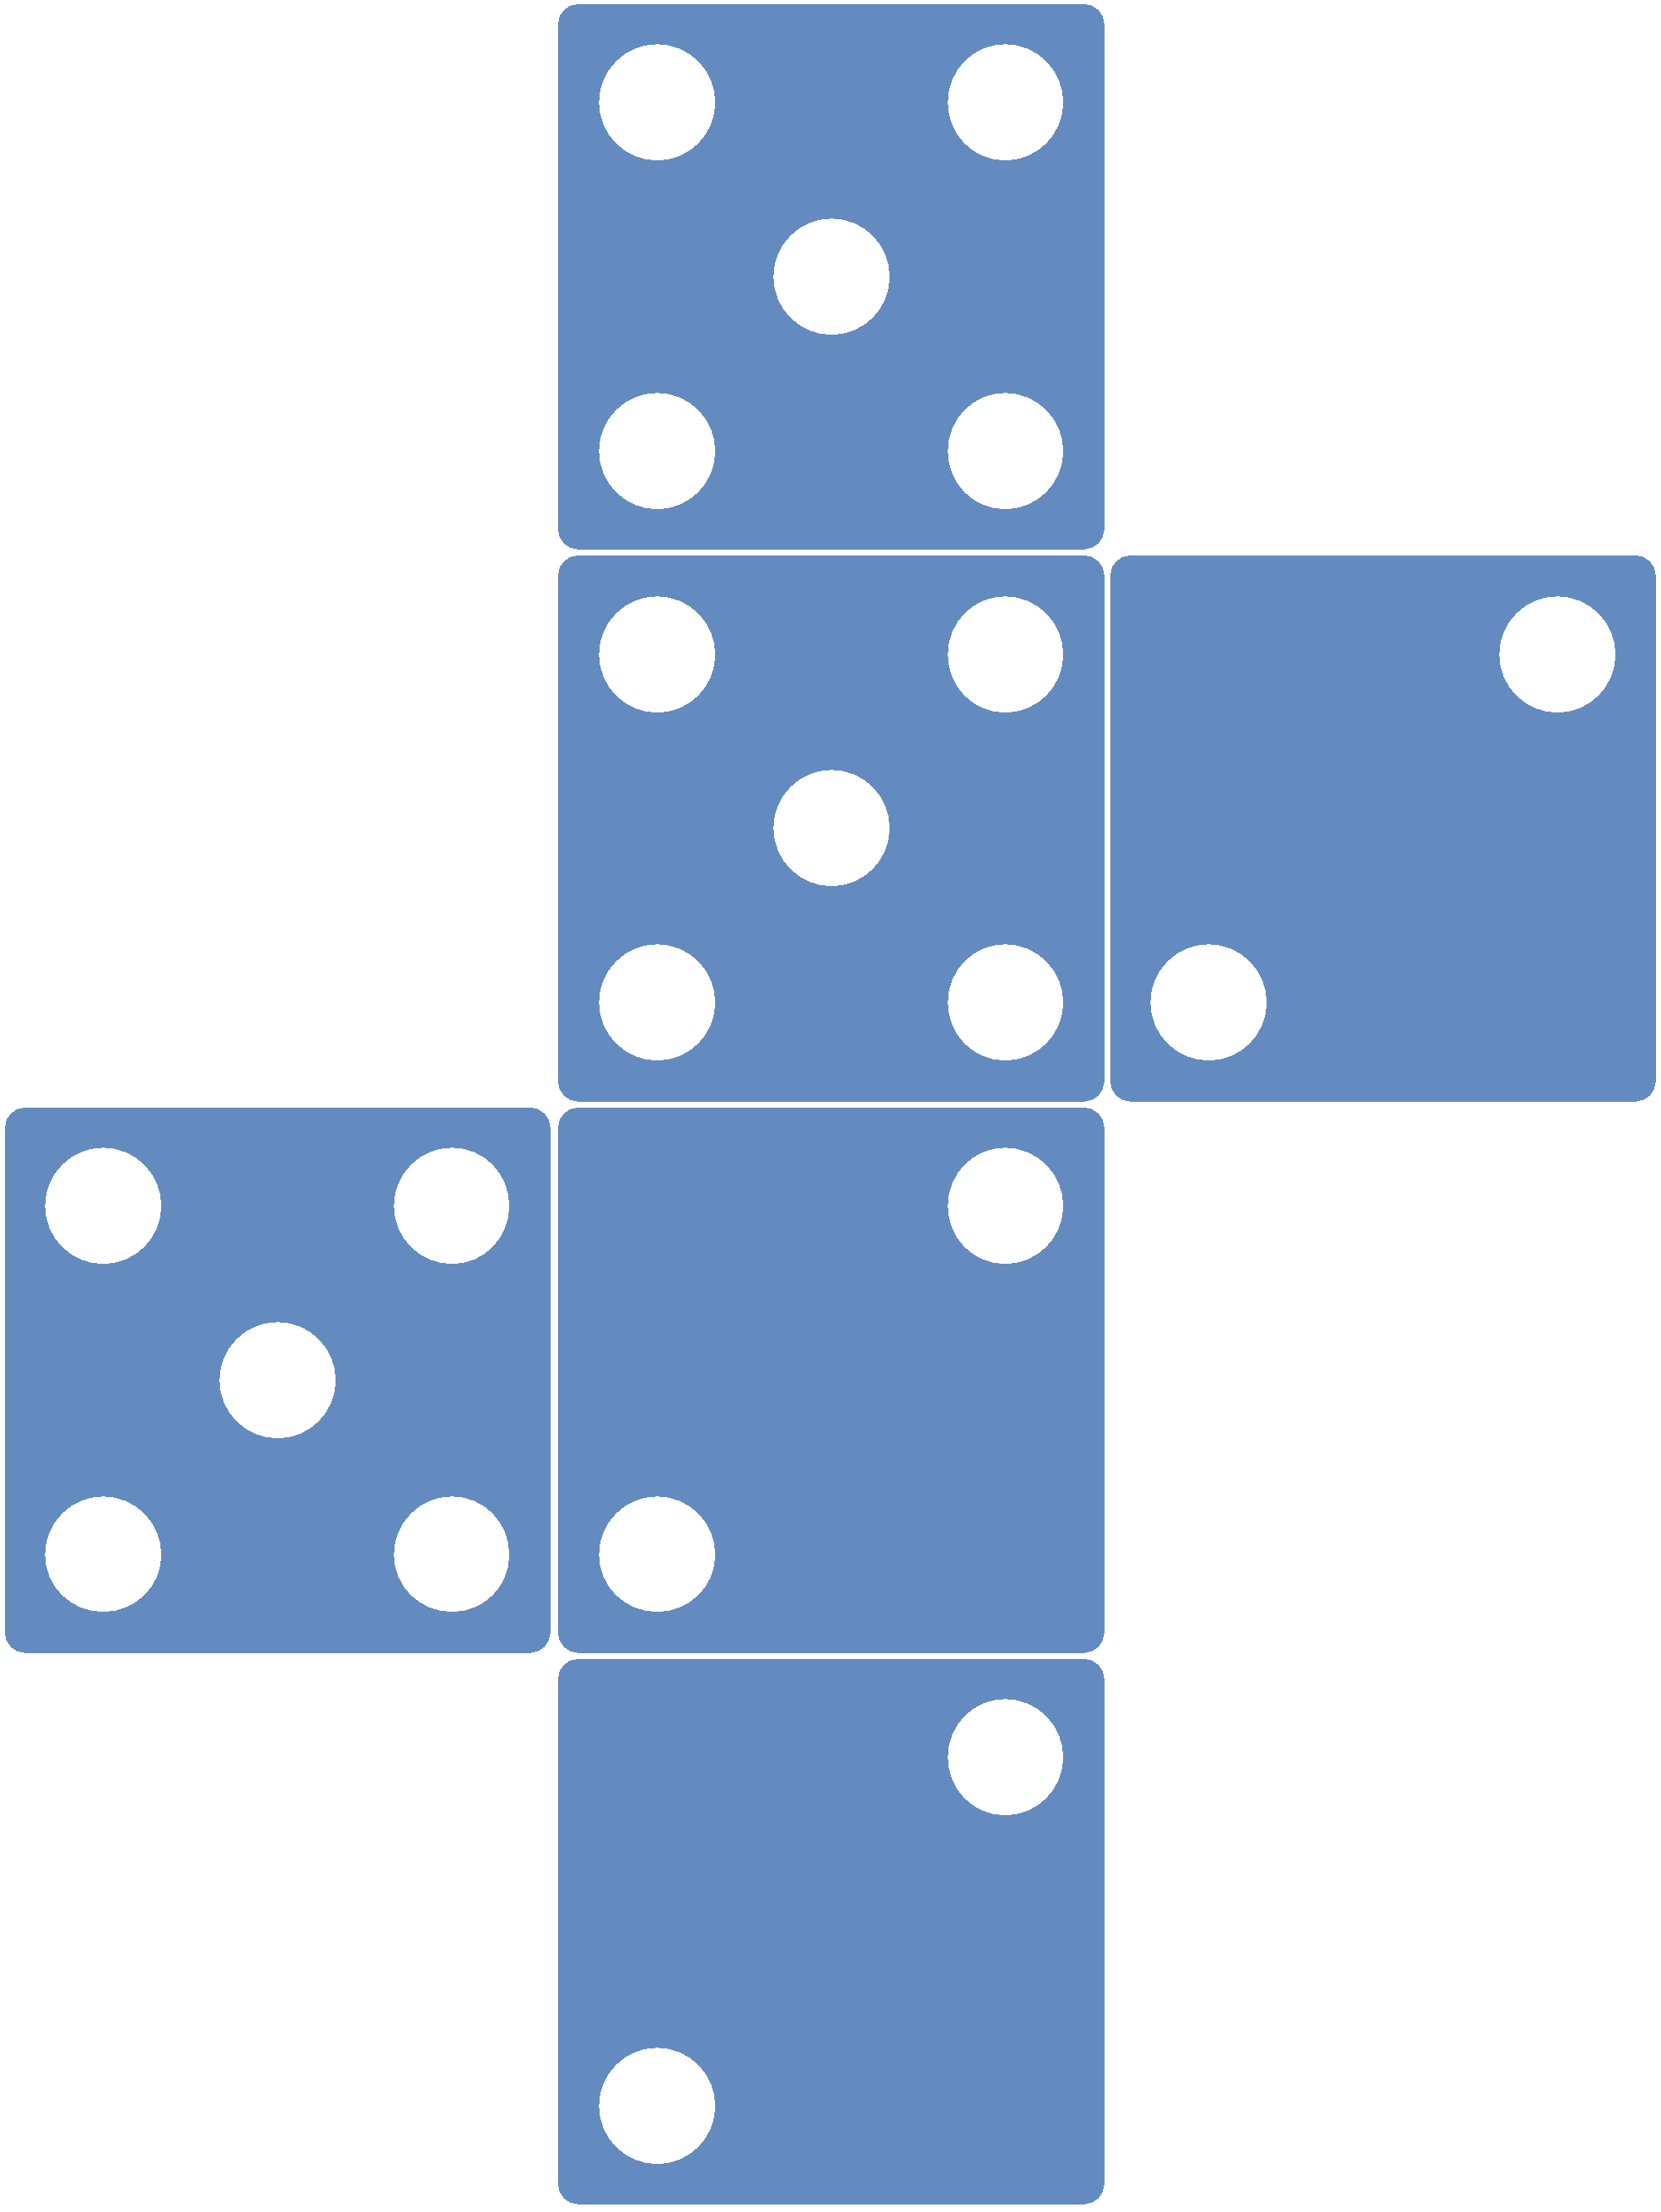
\includegraphics[width=4cm]{img/blue_die.png}
    \hspace{1cm}
    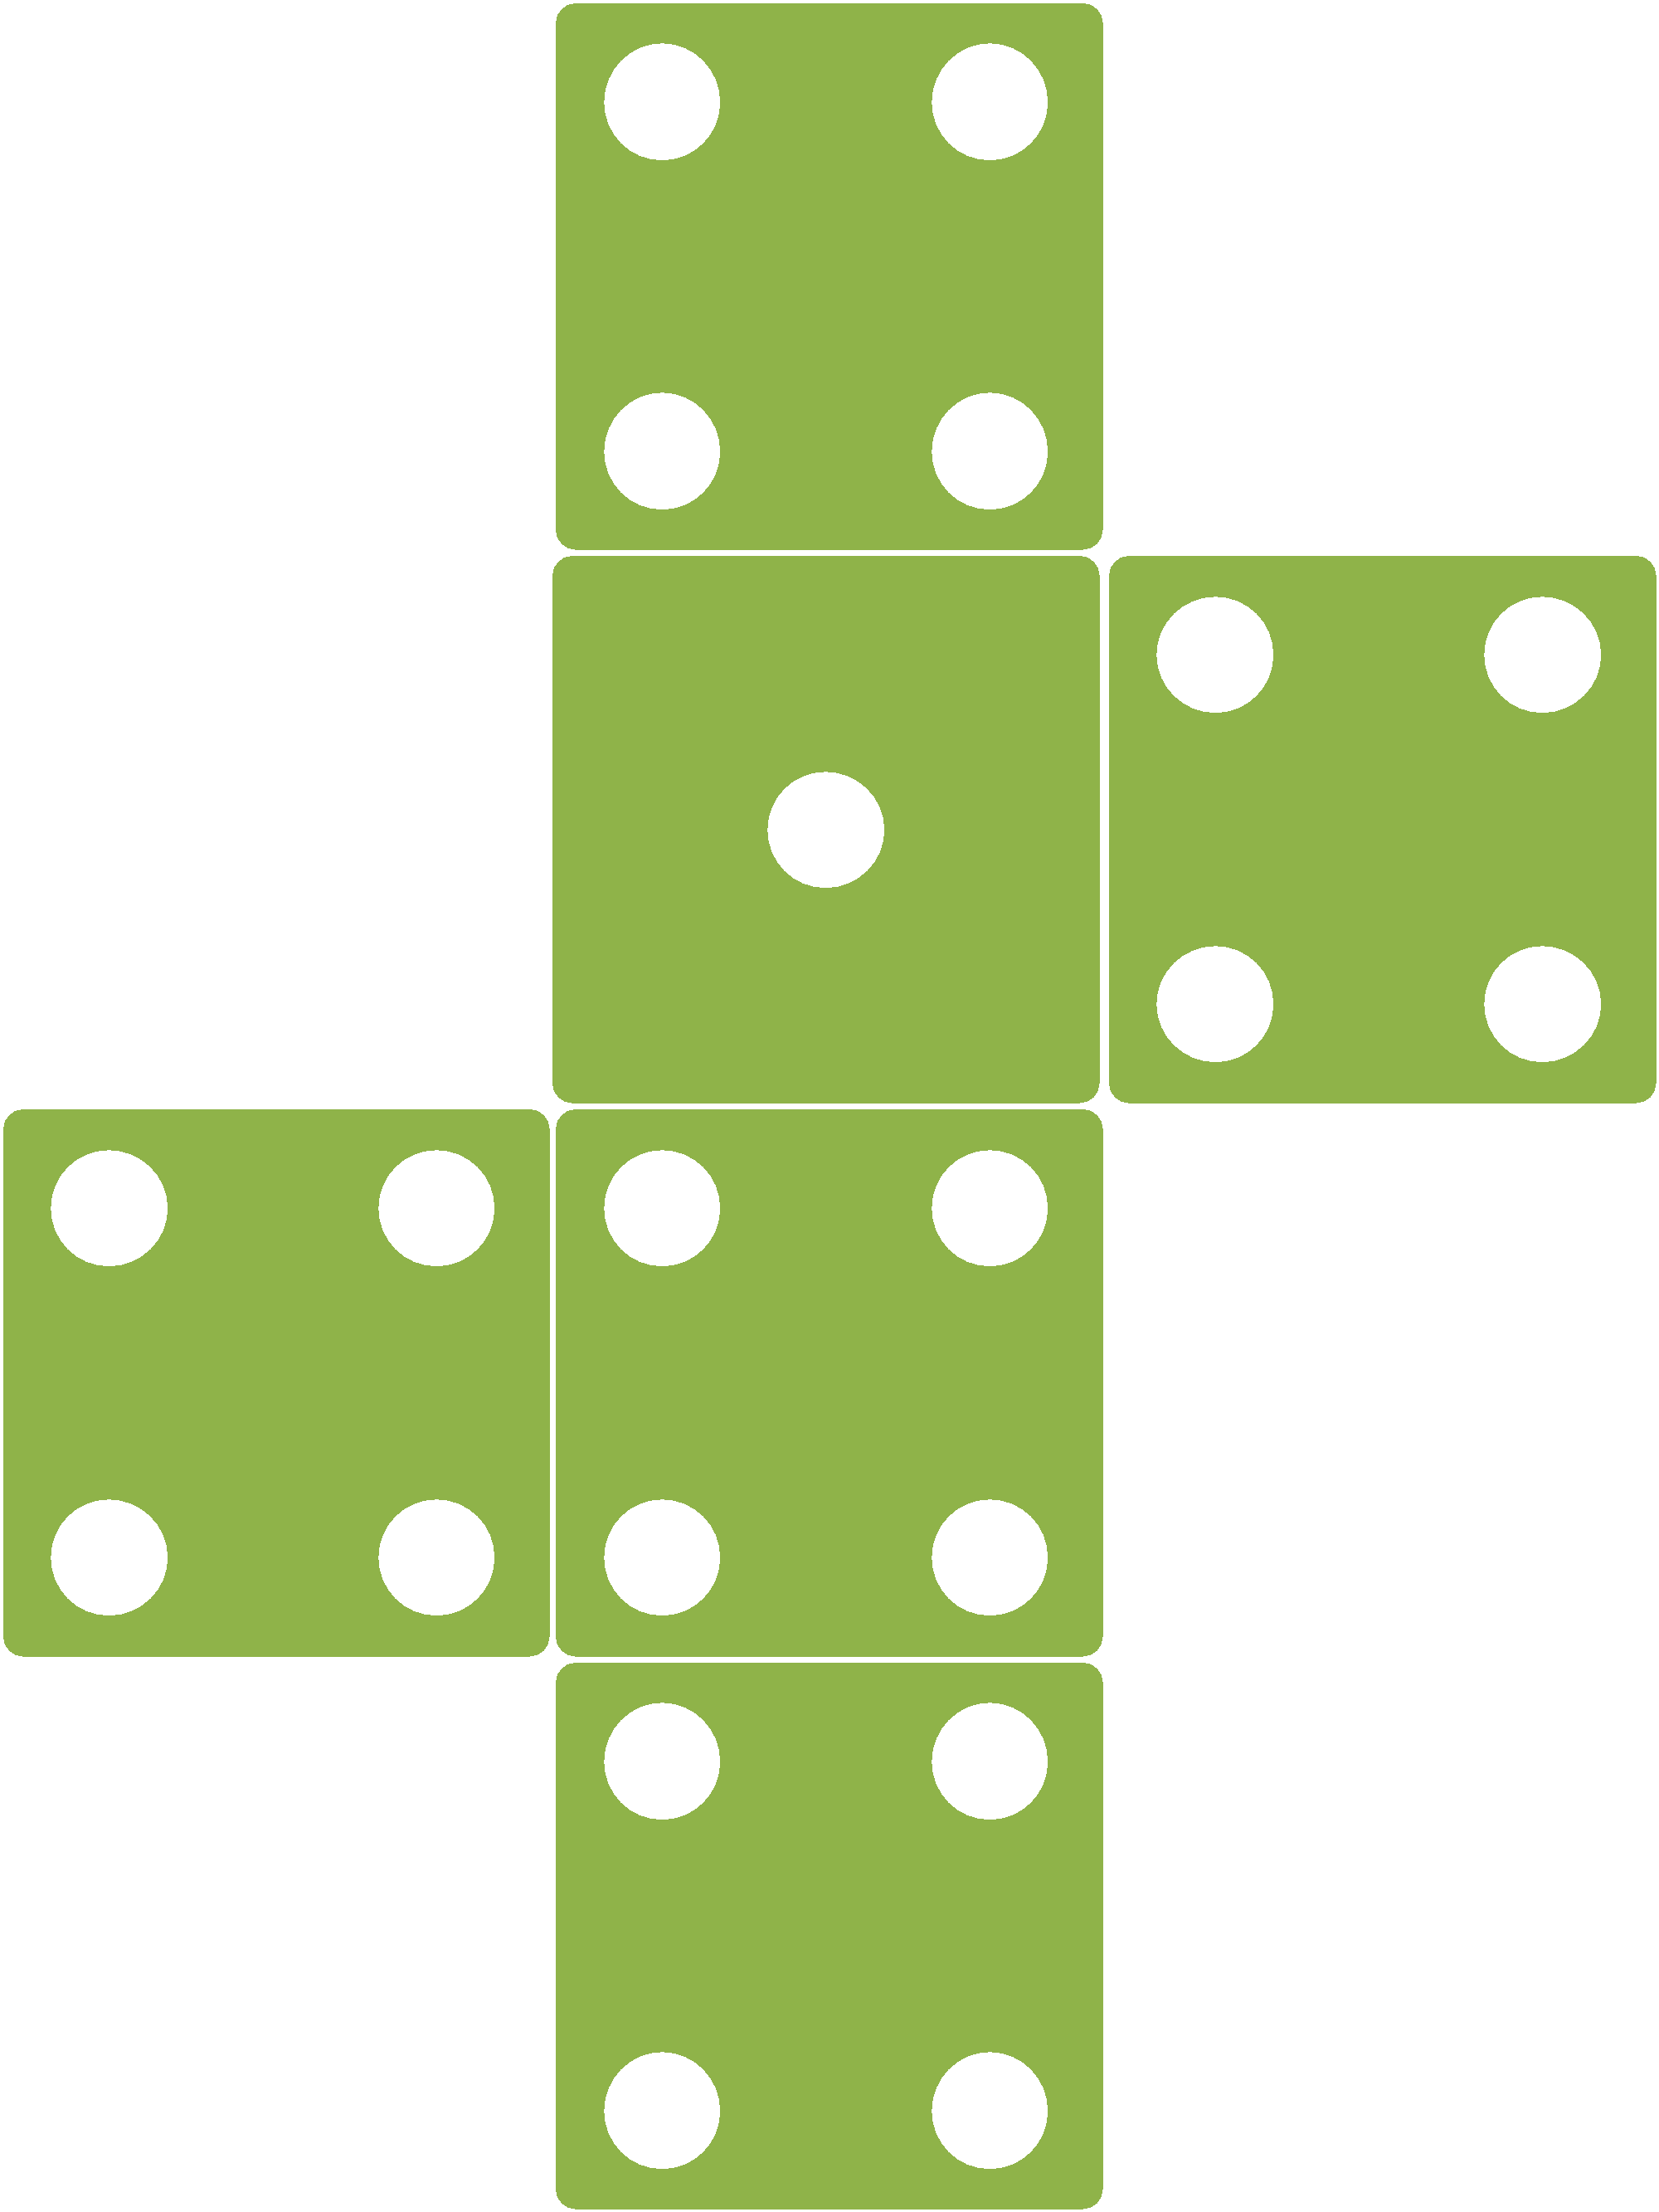
\includegraphics[width=4cm]{img/green_die.png}          
\end{center}
    
\question What is the mean value for the red die ?\\

\question What is the probability of the red die beating the blue die?\\

\question If your opponent choses the red die, which die would you choose?\\

\question Is one of the dice better than the other two ? Why/why not ?\\

\question Now consider a game in which we throw two red dice and two blue dice. We compare the total on the
two red dice and the total on the two blue dice in order to see who has won.\\
Draw a tree diagram to show the probabilities. At the first level, draw three branches for each possible total for the two red dice. At the second level of the tree, draw three branches for the totals of the two blue dice.\\

What is the probability of the blue dice beating the red dice? 

\begin{encadrecolore}{TODO}{UGLiBlue}
    \begin{itemize}
        \item Identify all the words and/or sentances which need to be defined or clarified.
        \item Find appropriate notations for all the relevant quantities of this problem.
        \item Prepare a 5 minute talk on your results, which you could present to the others.
    \end{itemize}
\end{encadrecolore}
\end{document}